\begin{frame}
    \begin{centering}
        \vskip5ex plus 1filll
        {\usebeamerfont{title page title}\usebeamercolor[fg]{title page} Harmonic Exciter\\[1.5ex]}
        \vskip0pt plus 1filll
    \end{centering}
\end{frame}

\begin{frame}{Harmonic Exciter}
    What is a harmonic exciter?\vspace{3ex}
    \begin{itemize}
        \item Add subtle harmonic distortion
        \item Make audio sound ``shiny'', ``brighter'', ``enhanced''
        \item Used for mixing, live broadcasts,
        restoring old recordings with missing spectral content
    \end{itemize}
\end{frame}

\begin{frame}{Aphex Aural Exciter\footcite{aphex}}
    \begin{figure}
        \centering
        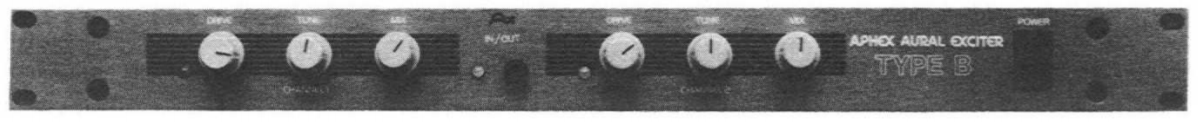
\includegraphics[width=4.25in]{Figures/aphex.png}
    \end{figure}
    \begin{itemize}
        \item Introduced in the mid-1970's
        \item Used by Jackson Browne, The Four Seasons, Linda Ronstadt, and more
        \item Originally rented to studios for \textbf{\$30 per minute}
    \end{itemize}
\end{frame}

\begin{frame}{Harmonic Exciter}
    Goals:
    \vspace{3ex}
    \begin{itemize}
        \item Exciter model that sounds ``smooth''
        \item Generalize the model to transcend circuit modelling\footcite{giannoulis2012digital}
    \end{itemize}
\end{frame}

\begin{frame}{Harmonic Exciter}
    \begin{figure}
        \centering
        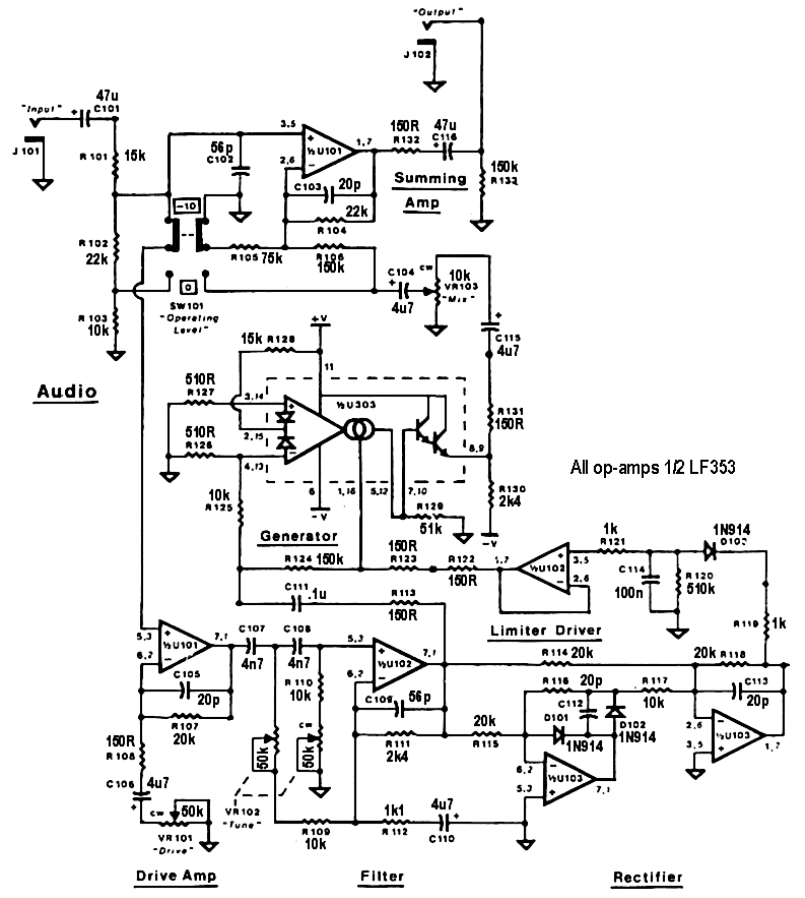
\includegraphics[height=2.5in]{Figures/exciter_circuit.png}
    \end{figure}
\end{frame}

\begin{frame}{Harmonic Exciter}
    \begin{figure}
        \centering
        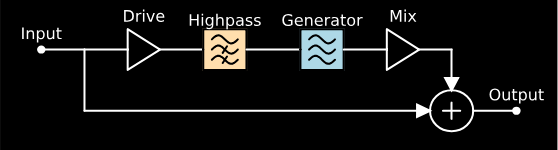
\includegraphics[width=4.25in]{../Exciter/Pics/Exciter_FullArch.png}
    \end{figure}
\end{frame}

\begin{frame}{Harmonic Exciter: Generator}
    \begin{figure}
        \centering
        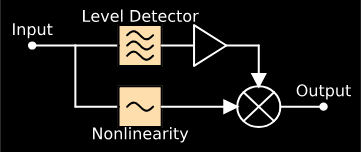
\includegraphics[width=4.25in]{../Exciter/Pics/Exciter_Arch.png}
    \end{figure}
\end{frame}

\begin{frame}{Harmonic Exciter: Level Detector}
    Rectifying nonlinearity \rightarrow LPF
    \begin{columns}
        \begin{column}{0.5\linewidth}
            \begin{figure}
                \centering
                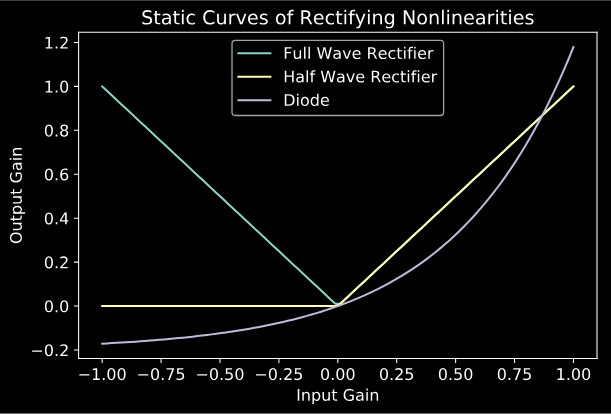
\includegraphics[width=2in]{../Exciter/Pics/rect_static}
            \end{figure}
        \end{column}
        \begin{column}{0.5\linewidth}
            \begin{figure}
                \centering
                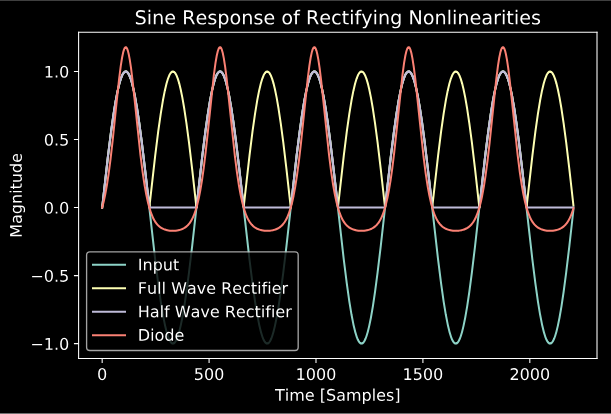
\includegraphics[width=2in]{../Exciter/Pics/rect_sine}
            \end{figure}
        \end{column}
    \end{columns}
\end{frame}

\begin{frame}{Harmonic Exciter: Level Detector}
    \begin{figure}
        \centering
        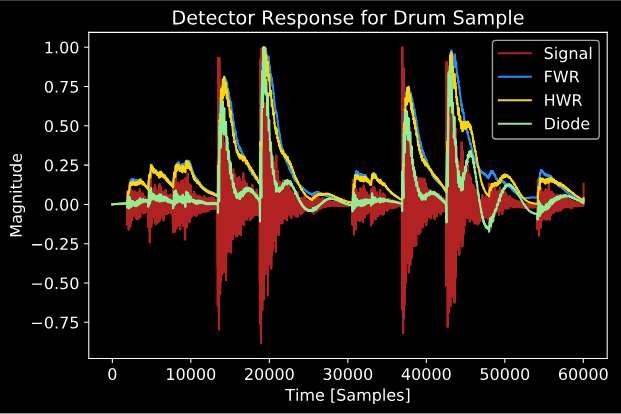
\includegraphics[height=2.5in]{../Exciter/Pics/Waveform_Detected.png}
    \end{figure}
\end{frame}

\begin{frame}{Harmonic Exciter: Nonlinearity}
    \begin{figure}
        \centering
        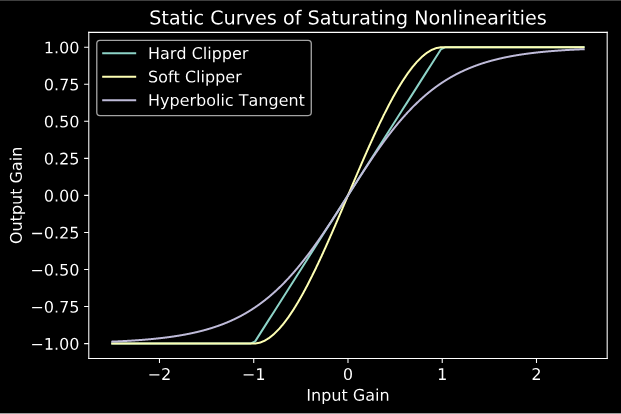
\includegraphics[height=2.5in]{../Exciter/Pics/saturating_static.png}
    \end{figure}
\end{frame}

\begin{frame}{Harmonic Exciter: Generator}
    \begin{figure}
        \centering
        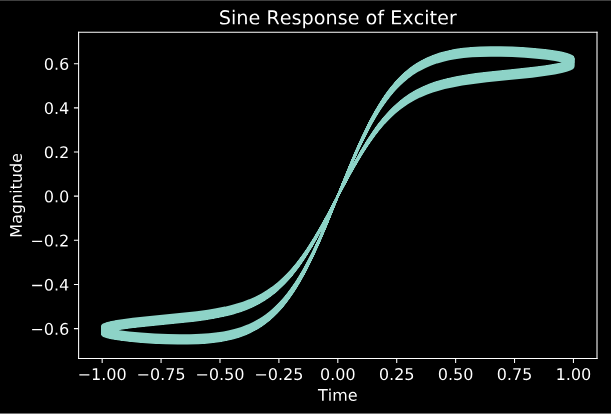
\includegraphics[height=2.5in]{../Exciter/Pics/exciter_static.png}
    \end{figure}
\end{frame}

\begin{frame}{Harmonic Exciter: Generator}
    \begin{figure}
        \centering
        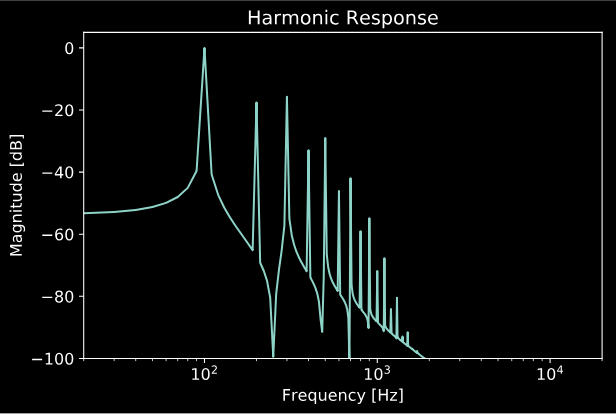
\includegraphics[height=2.5in]{../Exciter/Pics/exciter_harm.png}
    \end{figure}
\end{frame}
